\documentclass[a4paper,10pt]{article}

\usepackage[utf8]{inputenc}
%\usepackage[T1]{fontenc}

\usepackage{textcomp}           % Extra Symbole (Grad Celsius etc.)
\usepackage{amssymb,amsmath}    % Schöne Formeln (AMS = American Mathematical Society)
\usepackage{graphicx}           % Bilder und Seitenränder
\usepackage{subcaption}			% captions for subfigures
\usepackage{booktabs}           % Schönere Tabellen
\usepackage{colortbl}           % Farbige Tabellen

%\usepackage{tcolorbox}			% schöne bunte Boxen
\usepackage{mathtools}			% \mathclap für ordentliche \underbrace-			environments
\usepackage[left=2cm,right=2cm,top=2cm,bottom=2cm]{geometry}			% Pagelayout mit \newgeometry, \restoregeometry
\usepackage{float}
\usepackage{wrapfig}
\usepackage{enumitem}
\usepackage{float}
\usepackage{braket}
\usepackage{caption}
\usepackage[per-mode=fraction,output-decimal-marker={.},binary-units=true,separate-uncertainty=true]{siunitx}
\usepackage[breaklinks=true,colorlinks=true,linkcolor=blue,urlcolor=blue,citecolor=blue]{hyperref}
\usepackage{physics}
\usepackage{url}
\usepackage{subcaption}
\usepackage{calrsfs}
\DeclareMathAlphabet{\pazocal}{OMS}{zplm}{m}{n}
\usepackage{tikz}
\usetikzlibrary{decorations, positioning, intersections, calc, shapes,arrows, scopes}
\usepackage{pgfplots}
\usepackage{bodegraph}
\usepackage{circuitikz}
\usepackage{chemfig}
\usepackage{chemformula}
\usepackage[toc,page]{appendix}
\graphicspath{{./img/}}
\usepackage{verbatim}

\DeclareSIUnit\elementarycharge{e}

\newcommand{\dif}{\mathrm{d}}

\bibliographystyle{unsrtnat}

\renewcommand{\k}{\mathbf{k}}
\begin{document}
\begin{titlepage}
 \begin{center}
	\Large{Advanced laboratory course 3}
	\end{center}
	\begin{center}
	 \LARGE{\textbf{FP3 - Rare gas clusters}}
	\end{center}

	\begin{center}

	\large Marco \textsc{Canteri} \\
	marco.canteri@student.uibk.ac.at\\
	\large Maximilian Gerold \textsc{Münst} \\
	maximilian.muenst@student.uibk.ac.at
	\end{center}

	\begin{center}
	\vspace{1cm}
	Innsbruck, \today
	\vspace{1cm}
	\end{center}

	\begin{abstract}
	We created neon clusters via superbeam expansion technique, we then studied the isotope population of the clusters, magic numbers, and energy appearance. Moreover, we studied the 
	impact of air as pick-up gas in the neon clusters.
    \end{abstract}
    \vspace{1cm}

	\begin{center}
	
\includegraphics[scale=0.56]{img/uibk}
	\end{center}

\end{titlepage}


\section{Introduction}
In this experiment we explored the world of clusters, which are an aggregate of atoms with no particular structure. Cluster are the missing link between molecules and condensed matter, their wide applications are fundamental in nanotechnology, where clusters are the building blocks of the technology.

\section{Theoretical Background}

What's neon? And what's the meaning of a neon cluster? Can we reach god with it? Can we finally understand the meaning of life?\\
These and more questions will be answered in this section. You will be surprised that the answer is $42$. 

\subsection{Cluster formation}
There are different ways to produce clusters, however, usually those methods are built on 4 steps:
\begin{itemize}
	\item Vaporization (producing sufficiently cold particles in the gas phase)
	\item Nucleation (Condensation of gaseous atoms to form a cluster nucleus)
	\item Growth (adding particles to existing nuclei)
	\item Coalescence (Merging of small clusters) 
\end{itemize}
To start the formation of clusters the thermal energy has to be smaller than the binding energy of the cluster. To generate a dimer, i.e. a two atom cluster, a three body collision is necessary in order to conserve energy and momentum. 
\begin{equation}
	\ch{A} + \ch{A} + \ch{A} \rightarrow \ch{2 A} + \ch{A}
\end{equation}

\section{Experimental Setup}
Basically, the setup in this experiment has to first produce and grow clusters of Neon atoms and in a second step ionize said clusters. Finally the ionized clusters have to be detected. 

\subsection{Cluster source} 
In this setup cluster nuclei are generated by means of supersonic expansion of the source gas. Neon gas is stored in a stagnation chamber at roughly \SI{13}{\bar} and low temperature (about \SI{20}{\k}). It is then released into a vacuum chamber where the gas adiabatically expands at supersonic speed. It is noteworthy that the gas velocity is approximately constant during the expansion, but the quickly decreasing speed of sound gradually increases the local Mach number. \\
Fig. \ref{fig_expansion} shows a sketch of the expansion cone generated by the Neon gas. As there is a low but finite background pressure in the expansion chamber, two shock zones develop: a barrel shock, which is formed symmetrically around the central axis of the expansion zone and a termination shock at the end of the expansion region, referred to as the Mach disk. Together, these shock fronts shield what is called the zone of silence from the background gas, which means that there is hardly any collisions with the background gas to be expected in the zone of silence. The position of the Mach disk can be calculated as 
\begin{equation}
	\frac{x_\mathrm{M}}{d} = 0.67 \sqrt{\frac{p_0}{p_\mathrm{b}}}, 
\end{equation}
where $d$ is the diameter of the nozzle, $p_0$ and $p_\mathrm{b}$ represent the stagnation pressure and the background pressure. In Fig. \ref{fig_expansion} the Mach disk is depicted once for an undistorted case as a dash-dotted line and once distorted by a skimmer. \\
The skimmer collects the central component of the gas jet and guides it into the cluster chamber, where the clusters are formed by nucleation. It has to be placed with care, as if it is placed to close to the nozzle, one will see turbulences in the expansion, while placing it behind the Mach disk results in considerable loss in intensity, as the collisions with the background gas are to be expected. The formed clusters are subsequently collided with an electron beam, such that the neutral clusters are positively ionized via electron ionization. The ions now can be analyzed with a mass spectrometer, for this experiment we used a linear quadrupole mass spectrometer.\\
The electron beam is created by evaporation from a filament, the beam is focused with a set of electron lenses and filtered by energy with an hemispherical electron monochromator.

\begin{figure}[htp!]
	\centering
	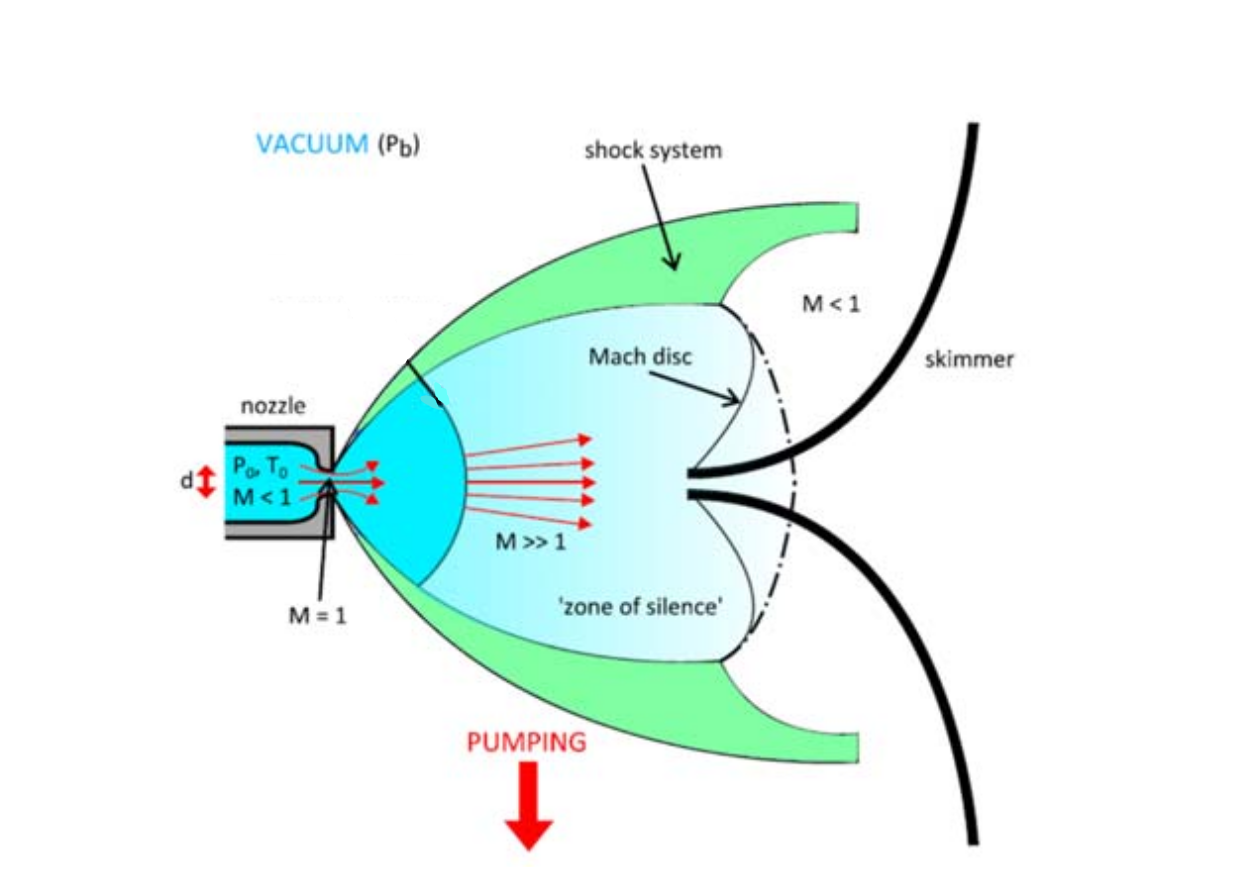
\includegraphics[width = 0.6 \textwidth]{expansion.png}
	\caption{Sketch of the expansion cone of the Neon gas. The figure was taken from \cite{script}. }
	\label{fig_expansion}
\end{figure}

\subsection{Electron monochromator}

As the set-up used in this experiment is used for actual research, we did not have to install or set up any components ourselves. All that had to be done was tune the voltages on several electrostatic lenses. 

As electron source a hairpin filament is used. However these electrons are emitted roughly isotropically in all directions, while their kinetic energy follows a Boltzmann distribution. A electric field now accelerates the electrons towards a set of electrostatic lenses meant to collimate the electron beam in a spatial direction. A layout of the structure is shown in Fig. \ref{setup}. 

The focused beam of electrons is then guided towards a hemispherical energy selector. As Fig. \ref{setup} indicates, this component is built up by two concentric hemispherical elements. By setting up a difference in voltage a electrostatic field is created. This way one can create an energy filter, as electrons which are too fast will collide with the outer element, while electrons that are too slow will be absorbed by the inner hemisphere. Variation of these two voltages allows for a variation of the energy of the electron beam, while maintaining a reasonably sharp energetic resolution. 

The energy filter is followed by a second set of electrostatic lenses, which spatially refocuses the flux of electrons into the collision chamber. The resulting ions are guided into the quadrupole mass filter, which measures the charge-mass-ratio, while remaining electrons are collected in the Faraday cup.

\begin{figure}[H]
	\centering
	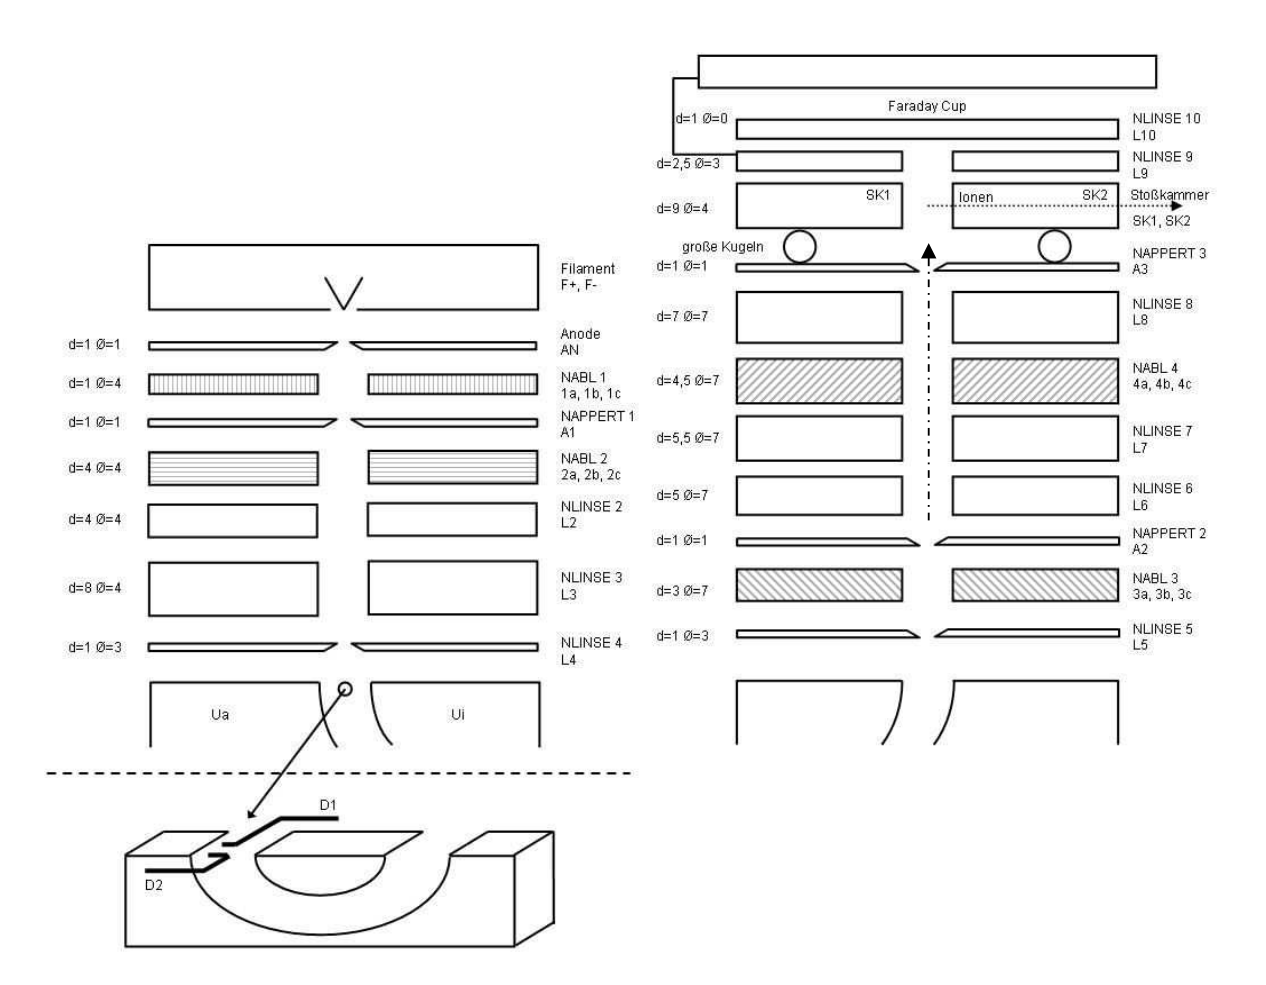
\includegraphics[width = 1 \textwidth]{setup.png}
	\caption{Layout of the used experimental setup, taken from \cite{script}. }
	\label{setup}
\end{figure}

\subsection{Quadrupole mass filter}
\section{Analysis}
\subsection{Isotope population}
In the first part of the experiment, we took a look at the isotope distribution of neon clusters. We analyzed the mass spectrum from 25 up to around 130 mass charge ratio, this should be enough to look for cluster with size up to \ch{Ne6+}. In figure \ref{isotopespectrum} the full spectrum can be seen. The first peak appears at around 28, this is not due Neon clusters, but from residual air in the setup, in fact air is most molecular nitrogen \ch{N_2} which has a weight of $\approx 28$ u. The other peaks are at 40, 60, 80, 100 and 120 which are respectively \ch{Ne_2+}, \ch{Ne_3+}, \ch{Ne_4+}, \ch{Ne_5+}, and \ch{Ne_6+}. For the isotope population we can take at look at the peak around 40. We can see two peaks at 40.5 and 42.5. The neon abundance is 90.92\% for \ch{^{20}Ne}, 8.82\% for \ch{^{22}Ne}, and 0.26\% for \ch{^{21}Ne} \cite{script}, therefore we expect the first peak to correspond to a neon dimer of two \ch{^{20}Ne}, and the second peak corresponding to a neon dimer made of one \ch{^{20}Ne} and one \ch{^{22}Ne}. However the values do not match exactly the theoretical prediction of respectively 39.98 and 41.98 \cite{umc}. Apparently there is a systematic error of 0.5, maybe due to the calibration of our linear quadrupole mass spectrometer. To further investigate this problem we can take a look at the measurement around 60, again there are two peaks at 60.5 and 62.5, these are due of \ch{Ne3+} first made of three \ch{^{20}Ne}, and then made of two \ch{^{20}Ne} and one \ch{^{22}Ne}, the calculated weight for this molecules are 59.98 and 61.98, again we see the same pattern of systematic error.

\begin{figure}[H]
	\centering
	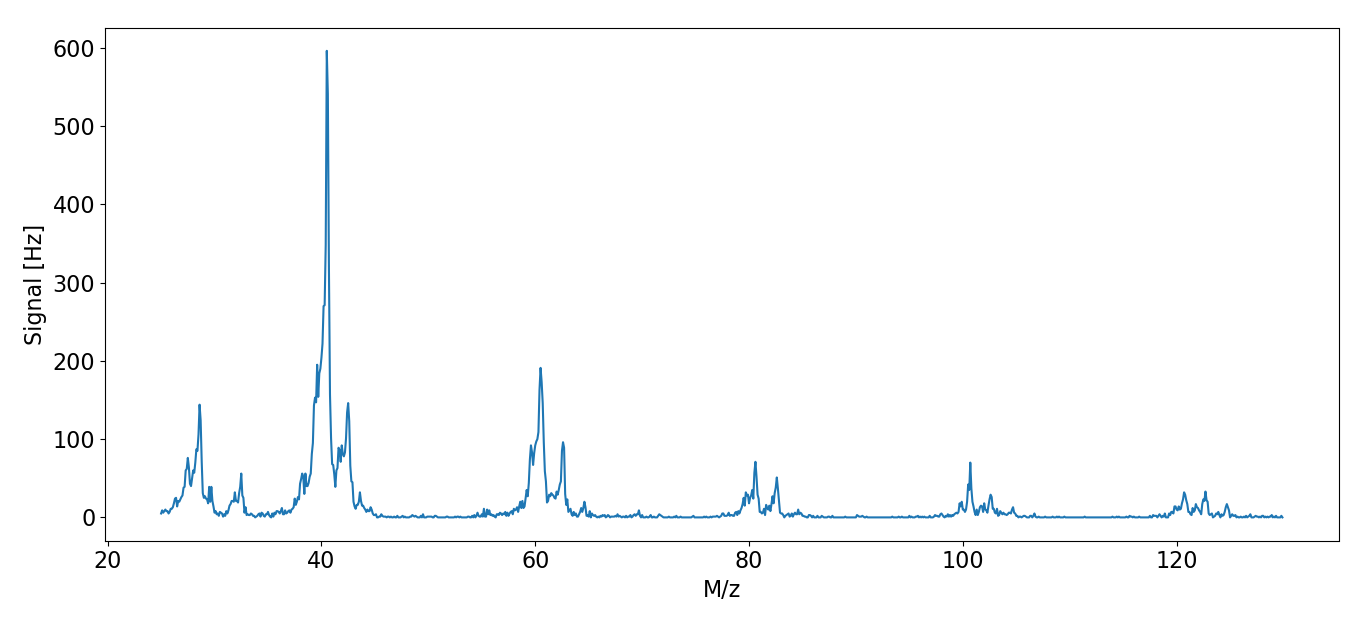
\includegraphics[width =\textwidth]{isotopespectrum}
	\caption{Mass spectrum of Neon clusters.}
	\label{isotopespectrum}
\end{figure}

\subsection{Magic numbers}
\subsection{Appearance energy for Ne and Ne$_2$}
\subsection{Pick-up}
\section{Conclusion}

\begin{thebibliography}{99}
\bibitem{script}
\textsc{Stephan Denifl}, \textit{FP3‐Praktikumsversuch – Edelgascluster/Rare gas clusters (SS 2018)}, 2018

\bibitem{umc}
\textsc{Matthias Letzel}, \textit{Universal Mass Calculator - Student Edition}, Universität Münster, \url{https://www.uni-muenster.de/Chemie.oc/ms/downloads.html}

\end{thebibliography}

\end{document}
